% !TEX root =  podc-submission.tex

\section{Queue Implementation} \label{DescriptQ}

\subsection{Overview of Implementation}
We use a \emph{tournament tree} to agree on a total ordering of the operations performed on the queue.
The tree is a static binary tree of height $\ceil{\log_2 p}$ with one leaf 
assigned to each process. 
Each tree node  stores an array of \emph{blocks}, where each block represents a 
sequence of enqueues and a sequence of dequeues.
In this section, we assume for simplicity that each node has an infinite blocks array.
Section \ref{reducing} describes how to replace the infinite array by a representation that uses bounded space.

To perform an operation on the queue, a process $P$ creates a block containing that single 
operation and appends it to the blocks array in $P$'s leaf.
Then, $P$ attempts to propagate the operation to each node along the path from that leaf to the root of the tree.
We shall define a total order on all operations that have been propagated to the root, which 
will serve as the linearization ordering of the operations.

To propagate an operation to a node $v$ in the tree, $P$ first observes
the blocks in both of $v$'s children that are not already in $v$,
creates a new block by combining information from those blocks, and attempts to append this 
new block to $v$'s blocks array using a CAS instruction.
Following \cite{}, we call this a 3-step sequence a
\op{refresh} on $v$. %(see Figure \ref{fig::propagstep}).
A successful \op{refresh} by $P$ may propagate pending operations by several other processes to $v$.
This cooperative approach is sufficient to ensure that if $P$ fails to CAS a 
new block into $v$'s array twice,
then its operation has been propagated to $v$ by some other process, so $P$ can continue 
onwards towards the root.

Now suppose $P$'s operation has been propagated all the way to the root.
If $P$'s operation is an enqueue, it has obtained a place in the linearization ordering and can terminate.
If $P$'s operation is a dequeue, $P$ must use information in the tree to compute the value that the
dequeue must return.  To do this, $P$ first determines which block in the root contains its operation
(since the operation may have been propagated to the root by some other process).
Then, $P$ determines whether the queue is empty when its dequeue is linearized. 
If so, it returns \nil\ and we call it a \emph{null dequeue}
If not, $P$ computes the rank\footnote{We say that the $r$th element in a sequence has rank $r$ within that sequence.} $r$ of its dequeue in the linearization ordering
among all non-null dequeues,
finds the $r$th enqueue in the linearization, and returns that enqueue's value.

The primary challenge is thus figuring out what information to store in each block so that 
the following tasks can be done efficiently (in a polylogarithmic number of steps).
\begin{enumerate}[label={(T\arabic*)}]
\item
\label{construct}
Construct a block for node $v$ that represents the operations contained in $O(p)$ consecutive blocks in $v$'s children, as required for a \op{refresh}.
\item
\label{findinroot}
Given a dequeue in a leaf that has been propagated to the root, find that operation's position in the root's blocks array.
\item
\label{findrank}
Given a dequeue's position in the root, determine whether it is a null dequeue (i.e., whether the queue is empty when it is linearized)
or determine the rank $r$ of the enqueue whose value it should return.
\item
\label{findenqueue}
Find the $r$th enqueue in the linearization ordering.
\end{enumerate}
Since these tasks depends on the linearization ordering, we describe that ordering next.

\subsection{Linearization Ordering}

An operation can terminate only after a block containing it has been appended to the root's blocks array.
So, if an operation $op_1$ terminates before another operation $op_2$ begins, 
$op_1$ will be in an earlier block than $op_2$ in root's blocks array.
Thus, our linearization orders operations according to the block they belong to in the root's blocks array.
Operations that appear in the same block are necessarily concurrent, so we can choose how to order them.

Each block in a leaf represents a single operation.
Each block $B$ in an internal node $v$ results from merging
several consecutive blocks from each of $v$'s children.
The blocks in $v$'s children are called the \emph{direct subblocks} of $B$.
A block $B'$ in a descendant of $v$ is a \emph{subblock} of $B$ if it is a direct subblock of $B$
or a subblock of a direct subblock of $B$.
A block $B$ represents the set of operations in all of $B$'s subblocks in leaves of the tree.

The operations propagated by a \op{refresh} are all pending when the \op{refresh} occurs,
so there is at most one operation per process.
Hence, a block represents at most $p$ operations in total.  
Moreover, we never append empty blocks, so 
each block represents at least one operation and it follows that a block can have at most $p$ direct subblocks.

As mentioned above, we are free to order operations within a block however we like.
For convenience, we order the enqueues and dequeues separately, and put the 
operations that were propagated from the left child before the operations from the right child.
More formally, we inductively define an sequence $E(B)$ of the enqueues represented by a block $B$.
If $B$ is a block in a leaf representing an enqueue operation, its enqueue sequence $E(B)$ is either the single
enqueue represented by the block (if $B$ stores an enqueue), or the empty sequence (if $B$ stores a dequeue).
If $B$ is a block in an internal node $v$ with direct subblocks $B^L_1, \ldots, B^L_\ell$ from the left child of $v$
and $B^R_1,\ldots,B^R_r$ from the right child of $v$, then $B$'s enqueue sequence is the concatenation $E(B^L_1)\cdots E(B^L_\ell)\cdot E(B^R_1) \cdots E(B^R_r)$.
The dequeue sequence $D(B)$ of a block $B$ is defined symmetrically.

Finally, if the root's blocks array contains blocks $B_1, \ldots, B_k$, the 
linearization ordering is 
$E(B_1)\cdot D(B_1) \cdot E(B_2) \cdot D(B_2) \cdots E(B_k) \cdot D(B_k)$.


\here{Need some figures illustrating tournament tree, ordering of operations, representation as blocks.  Might be able to modify Fig \ref{fig::set} and \ref{fig:block}.}

\begin{figure}[hbtp]
\begin{center}
\begin{tikzpicture} [level 1/.style={level distance=1.8cm,sibling distance=0.6cm}, level 2/.style={level distance=1.4cm,sibling distance=0.4cm}]
  
\Tree [.{$\big\{op_2^1,op_1^1,op_3^1\big\},\big\{op_4^1$, $op_3^2\big\},\big\{op_2^2, op_4^2\big\},\big\{op_1^2\big\}...$ }  [.{ $\big\{op_2^1, op_1^1\big\},\big\{op_2^2\big\},\big\{op_1^2\big\}...$ }
      {\begin{tabular}{|l|c|c|c}  \hline $op_1^1$ & $op_1^2$ & ... \\ \hline\end{tabular}} {\begin{tabular}{|l|c|c|c}  \hline $op_2^1$ & $op_2^2$ & ... \\ \hline \end{tabular}} ] [.{ $\big\{op_3^1\big\},\big\{op_4^1$, $op_3^2\big\},\big\{op_4^2\big\},...$ } {\begin{tabular}{|l|c|c|c}  \hline $op_3^1$ & $op_3^2$ & ... \\ \hline\end{tabular}} {\begin{tabular}{|l|c|c|c} \hline $op_4^1$ & $op_4^2$ & ... \\ \hline\end{tabular}} ] ]
\end{tikzpicture}
\caption[The operations merged in a \nf{Refresh} step with
  sets.]{\label{fig::set} Leaves are for processes $P_1$ to $P_4$ from
  left to right. In each internal node one can arbitrarily linearize
  the sets of concurrent operations  propagated together in a
  \nf{Refresh}. For example $op_4^1$ and $op_3^2$ have propagated
  together in one \nf{Propagate} step and they will be propagated up
  to the root together. Since their execution time intervals overlap,
  they can be linearized in any order.} 
\end{center}
\end{figure}

\begin{figure}[hbtp]
\begin{center}
\begin{tikzpicture}
[level 1/.style={level distance=3.3cm,sibling distance=0cm},
	level 2/.style={level distance=2.5cm,sibling distance=0cm},
	level 3/.style={level distance=1.7cm,sibling distance=2cm}]
\begin{small} 

\Tree [.{\begin{tabular}{|c|c|c|}  \hline (0,11) & (12,6) & (8,36) \\ \hline\end{tabular}}
 [.{\begin{tabular}{||c||c||}  \hline (10,2) & (5,3) \\\hline  \end{tabular}}
 [.{\begin{tabular}{||c|c||c||}\hline (2,3) & (4,1) & (0,5) \\\hline\end{tabular}} $\vdots$ $\vdots$ ]
  [.{\begin{tabular}{||c||c||}  \hline (0,2) & (1,2)  \\ \hline  \end{tabular}} $\vdots$ $\vdots$ ] ]
          [.{\begin{tabular}{||c||c||c|c||}  \hline (3,8) & (6,0) & (14,6) & (0,16) \\ \hline \end{tabular}}
           [.{\begin{tabular}{||c||c||c|c||}  \hline (0,3) & (4,2) & (5,1) & (3,5) \\ \hline \end{tabular}} $\vdots$ $\vdots$ ]
            [.{\begin{tabular}{||c|c||c||c||}  \hline (2,1) & (5,0) & (4,2) & (9,7) \\ \hline \end{tabular}} $\vdots$ $\vdots$ ] ] ]
\end{small}
\end{tikzpicture}
\end{center}
\caption[The operations merged in a \nf{Refresh} step with (left,
  right) blocks.]{\label{fig:block} Using blocks to represent
  operations. Blocks between two lines $||$ are propagated together to
  the parent. Each block consists of a pair (left, right) indicating
  the number of operations from the left and the right child,
  respectively. For example, (12,6) in the root contains  (10,2) from
  the left child and (6,0) from the right child. The third block in
  the root (8,36) is created by merging (5,3) from the left child and
  (14,6) and (0,16) from the right child. (5,3) is the superblock of
  (0,5) and (1,2) and (5,1),(3,5) and (4,2) are subblocks of (14,6).} 
\end{figure}

\subsection{Designing a Block Representation to Solve Tasks \ref{construct} to \ref{findenqueue}}

Each node has an infinite array called \var{blocks}.
To simplify the code, each node has an empty block in \var{blocks[0]}.
The node also has a \var{head} index which is the position in the \var{blocks} array to be used
for the next attempt to append a block to this node.

If a block contained an explicit representation of its sequences of enqueues and dequeues,
it would take $\Omega(p)$ time to construct a block, which would be much too slow for task \ref{construct}.
Instead, the block stores an implicit representation of the sequences.
We now explain how the fields of the blocks were chosen for this implicit representation. 
See Figure \ref{object-fields}.

A block in a leaf represents a single enqueue or dequeue.  The \var{element} field stores the value
enqueued for an enqueue operation, or \var{null} if the operation is a dequeue.

Each block in an internal node $v$ stores the indices of the last direct subblock in $v$'s left and right child in the fields \eleft\ and \eright.  This allows us to navigate to the direct subblocks of any block easily.
Blocks also store prefix sums of the numbers of enqueues and dequeues:
the block in $v.\var{blocks}[i]$ has two fields \var{sum\sub{enq}} and \var{sum\sub{deq}}
that store the total number of enqueues and dequeues in $v.\var{blocks[1..i]}$.
These fields allow us to pinpoint the exact location of an operation among the subblocks of a given block.
For example, consider finding the $r$th enqueue in the linearization ordering.
We use the \var{sum\sub{enq}} fields of the root's blocks to do a binary search
to locate which block in the root contains the operation.
If we know which block $B$ in some node $v$ contains the enqueue,
we can use the \var{sum\sub{enq}} field again determine which child of $v$ contains the enqueue
and then to do a binary search
among the direct subblocks of $B$ in that child.
Thus, we work our way down the tree until we find a leaf block, which explicitly stores 
the enqueue.
%Now, suppose we want to find the $r$th enqueue in the linearization ordering for task \ref{findenqueue}.Let $B_1, B_2, \ldots, B_k$ be the blocks in the root.
%First, we need prefix sums of the number of enqueues in $E(B_1)\cdot E(B_2)\cdots E(B_i)$
%so that we can do a binary search for the block $B_e$ that contains the $r$th enqueue.
%This prefix sum also allows us to know the rank $r'$ within $E(B_e)$ of the $r$th enqueue.
%Once we have $r'$, we need the number of enqueues that $B_e$ received from its left child
%to determine whether the enqueue came from the left or right child of the root.
%Suppose the enqueue came from the right child $v_r$.
%Then, we know that the index of the block in $v_r$ that contains the enqueue
%is between $B_{e-1}.\eright + 1$ and $B_e$.\eright.
%We can again do a binary search within this range.
%For this, we can again use the prefix sums of the number of enqueues in any prefix of the array $v_r.blocks$.
%We can then continue in this way down the tree until reaching a leaf where the enqueue is stored explicitly.
We shall show that the binary search in the root can be done in $O(\log p + \log q)$ steps,
and the binary search within each other node along the path to a leaf can be done in $O(\log p)$ steps,
for a total of $O(\log^2 p + \log q)$ steps to complete task \ref{findenqueue}.
All of the information needed for this search process can be derived from the 
\eleft, \eright\ and \var{sum\sub{enq}} fields.

To facilitate task \ref{findinroot}, each block has a field \var{super} that contains
the (approximate) index of its superblock in the parent node's blocks array.
We will ensure that this field's value differs from the true index of the superblock by at most 1.
This allows a process to determine the true location of the superblock by checking the \eleft\ or \eright\ values of just two blocks in the parent node.
Thus, starting from an operation in a leaf's block, one can use these indices to track the 
operation all the way up the path to the root, and determine the operation's location in a root block
in $O(\log p)$ time.

We now consider task \ref{findrank}.
First, we must determine whether the queue is empty when a dequeue occurs.
To facilitate this, each block in the root stores a \var{size} field that stores the number of elements
in the queue after all operations in the linearization ordering up to that block (inclusive) 
have been performed.
We can easily determine which dequeues in a block $B_d$ in the root are null dequeues using
$B_{d-1}.\var{size}$, which stores the size of the queue just before $B_d$'s operations are performed, and the number of enqueues and dequeues in $B_d$.
We can also compute the number of non-null dequeues in blocks $B_1, \ldots, B_{d-1}$ 
as $B_{d-1}.\var{sum\sub{enq}}-B_{d-1}.\var{size}$.
Then, for any non-null dequeue in $B_d$, we can also determine its
rank among all non-null dequeues in the linearization ordering, and hence the rank of the enqueue
whose value it should return (among all enqueues).

Now that we have defined the fields required for tasks \ref{findinroot}, \ref{findrank} and \ref{findenqueue},
we can easily see how to construct a new block $B$ during a \op{refresh} in $O(1)$ time.
A \op{refresh} on node $v$ reads the value $h$ of the \var{head} field of each of $v$'s children and stores 
$h-1$ in the $B.\eleft$ and $B.\eright$ fields of the new block.
Then, we can compute $B.\var{sum\sub{enq}}$ as $v.\var{left}.\var{blocks}[B.\eleft].\var{sum\sub{enq}} + v.\var{right}.\var{blocks}[B.\eright].\var{sum\sub{enq}}$.
For a block $B$ in the root, $B.\var{size}$ can be computed using the \var{size} field of the previous block,
the number of enqueues in $B$ and the number of non-null dequeues in $B$ (determined as described above).

The only remaining field is $B.\var{super}$.  When the block 
$B$ is created for a node $v$, we do not yet know where its
superblock will eventually be installed in $B$'s parent.
So, we leave this field blank.  After $B$ is installed 
in $v.\var{blocks[i]}$, processes cooperate to fill it in 
when they attempt to advance $v.\var{head}$ from $i$ to $i+1$.
They use the value read from the \var{head} field of $v$'s parent at that time.
As mentioned above, this might not be exactly the right index for $B$'s superblock, but we
shall prove that it is close.


\begin{figure}
\begin{algorithmic}[1]
\setcounter{ALG@line}{1}


\Statex $\diamondsuit$ \tt{\sl{Shared Variable}}
\begin{itemize}
\item \tt{\sl{Node} root} \sf{\com\ the root of a binary tree of \tt{Node}s with one leaf for each process}
\end{itemize}

\Statex $\diamondsuit$ \tt{\sl{Local Variable}}
\begin{itemize}
\item \tt{\sl{Node} leaf} \sf{\com\ process's leaf in the tree}
\end{itemize}

\Statex $\blacktriangleright$ \tt{\sl{Node}}
\begin{itemize}
\item \tt{\sl{Node} left, right, parent} \textsf{\com\ children and parent pointers initialized  when creating the tree}
\item \tt{\sl{Block[0..$\infty$]} blocks} \textsf{\com\ initially \tt{blocks[0]} contains an empty block with all integer fields equal to 0}
\item \tt{\sl{int} \head} \textsf{\com\ position to attempt appending next \tt{block} to \tt{blocks}, initially 1}
\end{itemize}

\Statex $\blacktriangleright$ \tt{\sl{Block}} 

\begin{itemize}
  \item \tt{\sl{int} super}
  \textsf{\com\ approximate index of the block's superblock in \var{parent.blocks}}
\end{itemize}



\Statex $\blacktriangleright$ \tt{\sl{InternalBlock} extends \sl{Block}} \sf{\com\ the following additional fields are used only for blocks in internal nodes}
\begin{itemize}
    \item \tt{int} \eleft, \eright
  \textsf{\com\ indices of the last subblock of the block in the left and right child}
  \item \tt{\sl{int} sum\sub{enq-left}}\textsf{\com\ number of enqueues in \tt{left.blocks[1..end\sub{left}]}}
  \item \tt{\sl{int} sum\sub{deq-left}}\textsf{\com\ number of dequeues in \tt{left.blocks[1..end\sub{left}]}}
  \item \tt{\sl{int} sum\sub{enq-right}}\textsf{\com\ number of enqueues in \tt{right.blocks[1..end\sub{right}]}}
  \item \tt{\sl{int} sum\sub{deq-right}}\textsf{\com\ number of dequeues in \tt{right.blocks[1..end\sub{right}]}}
\end{itemize}

\Statex $\blacktriangleright$ \tt{\sl{LeafBlock} extends \sl{Block}} \sf{\com\ the following additional fields are used only for blocks in leaves}
\begin{itemize}
  \item \tt{\sl{Object} element}
  \textsf{\com\ if the operation stored in the block is \tt{enqueue(x)} then \tt{element=x}, otherwise \tt{element=null}.}
  
    \item \tt{\sl{int} sum\sub{enq}, sum\sub{deq}}
  \textsf{\com\ number of enqueue, dequeue operations in  leaf's \var{blocks} array up to this block (inclusive)}
\end{itemize}

\Statex $\blacktriangleright$ \tt{\sl{RootBlock} extends \sl{InternalBlock}} \sf{\com\ the following field is used only for blocks in the root}
\begin{itemize}
  \item \tt{\sl{int} \size}%
  \textsf{\com\ size of the queue after performing all operations up to the end of this block in linearization order}
\end{itemize}

\end{algorithmic}
\caption{Objects used in Tournament Tree Data Structure \label{object-fields}}
\end{figure}

---------


In an execution on a queue where no dequeue operation returns
\nf{null}, the $k$th dequeue returns the argument of the $k$th
enqueue. In the general case a dequeue returns \nf{null} if and only
if the queue size after the previous operation is 0. We refer to such
a dequeue as a \it{null dequeue}. If the dequeue is the $k$th non-null
dequeue, it returns the argument of the $k$th enqueue. Having the size
of the queue after an operation we can compute the number of non-null
dequeues from the number of enqueues before the operation. So, if we
store the size of the queue after each block of operations in the
root, we can compute the index of the enqueue whose argument is the
response to a given dequeue in constant time. 

In our case of implementing a queue, a process only needs to compute
the rank of a \nf{Dequeue} and get an \nf{Enqueue} with a specific
position.  We know we can linearize operations in a block in any
order; here, we choose to put \nf{Enqueue} operations in a block
before \nf{Dequeue} operations. Consider the following operations,
where operations in a cell are concurrent. 
\begin{table}[hbtp]
\centering
\begin{small}
\begin{tabular}{c|c|c|c}
    \hline \texttt{Deq} & \texttt{Enq(5)}, \texttt{Enq(2)}, \texttt{Enq(1)}, \texttt{Deq}& \texttt{Enq(3)}, \texttt{Deq}&  \texttt{Enq(4)}, \texttt{Deq}, \texttt{Deq}, \texttt{Deq}, \texttt{Deq}\\ \hline
  \end{tabular}
\end{small}
\caption{An execution on a queue separated by the operations in the root blocks.}
\end{table}

\noindent The \texttt{Dequeue} operations return \texttt{null, 5, 2,
  1, 3, 4, null}, respectively. 
Now, we claim that by knowing the size of the queue, we can compute
the rank of the required \texttt{Enqueue} for any non-null
\nf{Dequeue}. We apply this approach to blocks; if we store the size
of the queue after each block of operations, we can compute the index
of each \nf{Dequeue}'s result in \textsc{O}$(1)$ steps. 

\begin{table}[hbtp]
\centering
\begin{small}
  \begin{tabular}{c|c|c|c|c}
    \hline &\texttt{Deq} & \texttt{Enq(5)}, \texttt{Enq(2)}, \texttt{Enq(1)}, \texttt{Deq}& \texttt{Enq(3)}, \texttt{Deq}&  \texttt{Enq(4)}, \texttt{Deq}, \texttt{Deq}, \texttt{Deq}, \texttt{Deq}\\ \hline
    \#\tt{Enq}s & 0 & 3 & 1 & 1 \\ \hline
    \#\tt{Deq}s & 1 & 1 & 1 & 4 \\ \hline
    Size at end & 0 & 2 & 2 & 0 \\ \hline
  \end{tabular}
\end{small}
  \caption{Augmented history of operation blocks on the queue.}
\end{table}

\noindent The size of the queue after the $b$th block in the root
could be computed as 
$$\textrm{max}\Big(\textrm{size after }(b-1)\textrm{th block} +
\#\textrm{\tt{Enqueue}s in }b\textrm{th block} -
\#\textrm{\tt{Dequeue}s in }b\textrm{th block}, 0\Big).$$ 
\noindent Moreover, the total number of non-null dequeues in blocks
$1,2,...,b$ in the root is 
$$ \sum_{i=1}^{b} \#\textrm{\tt{Enqueue}s in }i\textrm{th block} -
\textrm{size after }b\textrm{th block}.$$ 

Given a \texttt{Dequeue} is in block $B$, its response is the argument
of the \tt{Enqueue} whose rank is 
\begin{center}
    \#\textrm{non-null } \nf{Dequeue}s in  blocks $1,2,...,b-1 +  $index of the \nf{Dequeue} among B\textrm{'s} \nf{Dequeue}
\end{center}
if \vspace{-3em}
\begin{center}
    $\big ($size of the queue after $b-1\textrm{th block} + \#\textrm{\tt{Enqueue}s in }b\textrm{th block} $\\$- \textrm{index of \tt{Dequeue} in }B\textrm{'s \tt{Dequeue}s} \big )\geq 0$.
\end{center}
Otherwise, the response would be \nf{null}.


\subsection{Details of the Implementation}
Section \ref{algQ} gives the pseudocode for the queue
implementation. It uses the following two types of objects. 
\paragraph{\tt{Node}} 
 In each \texttt{Node} we store pointers to its parent and its left
 and right child, an array of \nf{Block}s called \texttt{block}s and
 the index \nf{head} of the first empty entry in \texttt{blocks}. 

\paragraph{\tt{Block}}
 The information stored in a \nf{Block} depends on whether  the
 \nf{Block} is in an internal node or a leaf. If it is in a leaf, we
 use a \nf{LeafBlock} which stores one operation. If a block $B$ is in
 an internal node $n$, then it contains subblocks in the left and
 right children of $n$. The left subblocks of $B$ are some consecutive
 blocks in the left child of $n$ starting from where the left
 subblocks of the block prior to $B$ ended. The right subblocks of $B$
 are defined similarly. In each \texttt{block} we store four essential
 fields that implicitly summarize which operations are in the block
 \texttt{sum\textsubscript{enq-left}},
 \texttt{sum\textsubscript{deq-left}},
 \texttt{sum\textsubscript{enq-right}},
 \texttt{sum\textsubscript{deq-right}}. The
 \texttt{sum\textsubscript{enq-left}} field is the total number of
 \nf{Enqueue} operations in the blocks before the last subblock of $B$
 in the left child. The other fields' semantics are similar. The
 \nf{end\sub{left}} and \nf{end\sub{right}} field store the index of
 the last subblock of a block in the left and the right child,
 respectively. The approximate index of the superblock of non-root
 blocks is stored in their \nf{super} field. The \texttt{size} field
 in a block in the root node stores the size of the queue after the
 operations in the block have been performed.  

We now describe the routines used in the implementation.

\paragraph{\tt{Enqueue($e$)}}
An \nf{Enqueue} operation does not return a response, so it is
sufficient to propagate the \nf{Enqueue} operation to the root and
then use its position in the linearization for future \nf{Dequeue}
operations. \nf{Enqueue($e$)} creates a \nf{LeafBlock} with
$\nf{element}=e$, sets its \nf{sum\sub{enq}} and \nf{sum\sub{deq}}
fields and then appends it to the tree. 

\paragraph{\tt{Dequeue()}}
\nf{Dequeue} creates a \nf{LeafBlock}, sets its \nf{sum\sub{enq}} and
\nf{sum\sub{deq}} fields and appends it to the tree. Then, it computes
the position of the appended \nf{Dequeue} operation in the root using
\nf{IndexDequeue} and after that finds the response of the
\nf{Dequeue} by calling \nf{FindResponse}. 

\paragraph{\tt{Append($B$)}}
The \nf{head} field is the index of the first empty slot in
\nf{blocks} in a \nf{LeafBlock}. There are no multiple write accesses
on \nf{head} and \nf{blocks} in a leaf because only the process that
the leaf belongs to appends to it. \nf{Append($B$)} adds $B$ to the
end of the \nf{blocks} field in the leaf, increments \nf{head} and
then calls \nf{Propagate} on the leaf's \nf{parent}. When
\nf{Propagate} terminates, it is guaranteed that the appended block is
a subblock of a block in the \nf{root}.  

\paragraph{\tt{Propagate()}}
\nf{Propagate} on node $n$ uses the double refresh idea described
earlier and invokes two \nf{Refresh}es on $n$ in Lines
\ref{firstRefresh} and \ref{secondRefresh}. Then, it invokes
\nf{Propagate} on \nf{$n$.parent} recursively until it reaches the
root.  

\paragraph{\tt{Refresh()} and \tt{Advance()}}
The goal of a \nf{Refresh} on node $n$ is to create a block of $n$'s
children's new blocks and append it to $n$\nf{.blocks}. The variable
\nf{h} is read from $n$\nf{.head} at Line \ref{readHead}. The new
block created by \nf{Refresh} will be inserted into
$n\nf{.blocks[h]}$. Lines \ref{startHelpChild1}--\ref{endHelpChild1}
of \nf{$n$.Refresh} help to \nf{Advance} $n$'s children. \nf{Advance}
increments the children's \nf{head} if necessary and sets the
\nf{super} field of their most recently appended blocks. The reason
behind this helping is explained later when we discuss
\nf{IndexDequeue}. After helping to \nf{Advance} the children, a new
block called \nf{new} is created in Line
\ref{invokeCreateBlock}. Then, if \nf{new} is empty, \nf{Refresh}
returns \nf{true} because there are no new operations to propagate,
and it is unnecessary to add an empty block to the tree. Later we will
use the fact that all blocks contain at least one operation. Line
\ref{cas} tries to install \nf{new}. If it was successful, all is
good. If not, it means someone else has already put a block in
$n$\nf{.blocks[h]}. In this case, \nf{Refresh} helps advance
$n$\nf{.head} to \nf{h+1} and update the \nf{super} field of
$n$\nf{.blocks[h]} at Line \ref{advance}. 


\paragraph{\tt{CreateBlock()}} \texttt{$n$.CreateBlock($h$)} is used
by \nf{Refresh} to construct a block containing new operations of
$n$'s children. 
The block \nf{new} is created in Line \ref{initNewBlock} and its
fields are filled similarly for both left and right directions. The
variable  \nf{index\sub{prev}} is the index of the block preceding the
first subblock in the child in direction \nf{dir} that is aggregated
into \nf{new}. Field \texttt{new.end\textsubscript{dir}} stores the
index of the rightmost subblock of \nf{new} in the child. Then
\nf{sum\sub{enq-dir}} is computed from the sum of the number of
\nf{Enqueue} operations in the \nf{new} block from direction \nf{dir}
and the value stored in \texttt{$n$.blocks[h-1].sum\sub{enq-dir}}. The
field \nf{sum\sub{deq-dir}} is computed similarly. Then, if \nf{new}
is going to be installed in the \nf{root}, the \nf{size} field is also
computed. 

\paragraph{\tt{IndexDequeue($b,i$)}}

A call to $n$\nf{.IndexDequeue($b,i$)} computes the block and the rank
within the block in the root of the $i$th \nf{Dequeue} of the $b$th
block of $n$. Let $R_n$ be the successful  \nf{Refresh} on node $n$
that did a successful \nf{CAS(null, $B$)} into \nf{n.blocks[$b$]}. Let
$par$ be $n$\nf{.parent}. Without loss of generality, assume for the
rest of this section that ${n}$ is the left child of $par$. Let
$R_{par}$ be the first successful \nf{$par$.Refresh} that reads some
value greater than ${b}$ for \nf{left.head} and therefore contains
${B}$ as a subblock of its created block in Line
\ref{invokeCreateBlock}. Let $j$ be the index of the block that
$R_{par}$ puts in $par$\nf{.blocks}. 
 
Since the index of the superblock of ${B}$ is not known until $B$ is
propagated, $R_n$ cannot set the \nf{super} field of ${B}$ while
creating $B$. One approach for $R_{par}$ is to set the \nf{super}
field of ${B}$ after propagating $B$ to $par$. This solution would not
be efficient because there might be up to $p$ subblocks that $R_{par}$
propagated, which need to update their \nf{super} field. However,
intuitively, once $B$ is installed, its superblock is going to be
close to \nf{$n$.parent.head} at the time of installation. If we know
the approximate position of the superblock of $B$ then we can search
for the real superblock when it is needed. Thus, \nf{$B$.super} does
not have to be the exact location of  the superblock of $B$, but we
want it to be close to $j$. We can set \nf{$B$.super} to
\nf{$par$.head} while creating $B$, but the problem is that there
might be many \nf{Refresh}es on $par$ that could happen after $R_n$
reads $par$\nf{.head} and before propagating $B$ to $par$. If $R_n$
sets \nf{$B$.super} to \nf{$par$.head} after appending $B$ to
\nf{$n$.blocks} (Line \ref{setSuper1}), $R_n$ might go to sleep at
some time after installing $B$ and before setting \nf{$B$.super}. In
this case, the next \nf{Refresh}es on $n$ and $par$ help fill in the
value of \nf{$B$.super}. 

Block $B$ is appended to \nf{$n$.blocks[$b$]} on Line \ref{cas}. After
appending $B$, \nf{$B$.super} is set on Line \ref{setSuper1} of a call
to \nf{Advance} from \nf{$n$.Refresh} by the same or another process
or by Line \ref{helpAdvance} of a \nf{$n$.parent.Refresh}. We shall
show that this is sufficient to ensure that \nf{$B$.super} differs
from the index of $B$'s superblock by at most~1. 

\paragraph{\tt{FindResponse($b, i$)}}
To compute the response of the $i$th \nf{Dequeue} in the $b$th block
of the root Line \ref{checkEmpty} computes whether the queue is empty
or not. If there are more \nf{Dequeue}s than \nf{Enqueue}s the queue
would become empty before the requested \nf{Dequeue}. If the queue is
not empty, Line \ref{computeE} computes the rank $e$ of the
\nf{Enqueue} whose argument is the response to the
\nf{Dequeue}. Knowing the response is the $e$th \nf{Enqueue} in the
root (which is before the $b$th block), we find the block and position
containing the \nf{Enqueue} operation using \nf{DoublingSearch} and
after that \nf{GetEnqueue} finds its \nf{element}. 

\paragraph{\tt{GetEnqueue($b,i$)} and \tt{DoublingSearch($e, end$)}}
We can describe an operation in a node in two ways: the rank of the
operation among all the operations in the node or the index of the
block containing the operation in the node and the rank of the
operation within that block. If we know the block and rank within the
block of an operation, we can find the subblock containing the
operation and the operation's rank within that subblock in poly-log
time. To find the response of a \nf{Dequeue}, we know about the  rank
of the response \nf{Enqueue} in the root (\nf{e} in Line
\ref{computeE}). 
We also know the \nf{e}th \nf{Enqueue} is in
\nf{root.blocks[1..end]}. \nf{DoublingSearch} uses doubling to find
the range that contains the answer block (Lines
\ref{dsearchStart}--\ref{dsearchEnd}) and then tries to find the
required indices with a binary search (Line
\ref{dsearchBinarySearch}). 
A call to \nf{$n$.GetEnqueue($b,i$)} returns the \nf{element} of the
$i$th enqueue in the $b$th block of $n$. The range of subblocks of a
block is determined using the \nf{end\sub{left}} and
\nf{end\sub{right}} fields of the block and its previous block. Then,
the subblock is found using binary search on the \nf{sum\sub{enq}}
field (Lines \ref{leftChildGet} and \ref{rightChildGet}). 

